\section{Confronto delle tecniche di compilazione}
Storicamente le performance delle applicazioni Java sono sempre state molto criticate. Java è stato progettato per essere interpretato e portabile: i primi runtime avevano performance significativamente più basse dei concorrenti. Nel corso degli ultimi anni, però, i runtime Java hanno introdotto compilatori dinamici molto sofisticati: i compilatori JIT. Questi compilano selettivamente i metodi più frequentemente eseguiti in codice nativo durante l'esecuzione. Il fatto di compilare i metodi durante l'esecuzione, e non allo start-up, mantiene la portabilità. Grazie a questo, inoltre, le performance risultano incredibilmente migliorate. 

\subsection{Compilazione Just-in-time}
Figura~\ref{fig:jit} mostra un esempio di compilazione just-in-time. 
\begin{figure}
	\centering
	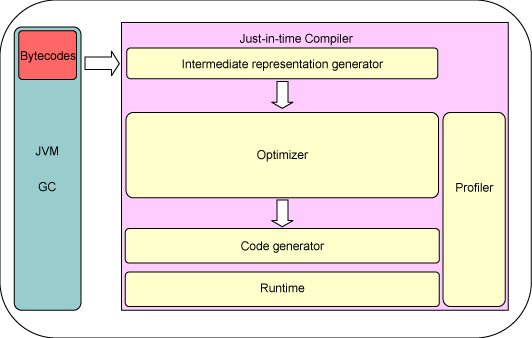
\includegraphics[width=0.7\linewidth]{jvmjit}
	\caption[Compilatore JIT]{Compilatore JIT}
	\label{fig:jit}
\end{figure}
I programmi Java vengono compilati un metodo alla volta mentre eseguono, per raggiungere performance migliori. Durante il processo viene generata una rappresentazione interna del metodo (differente dal bytecode, ma ad un livello più alto delle istruzioni macchina). Il compilatore poi esegue una serie di ottimizzazioni per migliorare la qualità e l'efficienza del codice finale e infine traduce tutto in istruzioni macchina del processore in uso. Il compilatore opera in un thread differente cosicché l'applicazione non è costretta a bloccarsi in attesa della fine della compilazione. Un framework (\texttt{Profile}) osserva il comportamento del programma per identificare i metodi eseguiti più frequentemente. 

L'eseguire la compilazione concorrentemente all'esecuzione mantiene l'indipendenza dalla piattaforma, ma ad un costo: il tempo richiesto per compilare si somma al tempo richiesto per l'esecuzione. Ci sono due soluzioni al problema:
\begin{itemize}
	\item compilare tutto il codice senza però effettuare analisi o ottimizzazioni costose (per mantenere veloce il processo). L'overhead in questo caso è talmente piccolo che è completamente recuperato dall'incremento di performance; 
	\item compilare solo metodi eseguiti veramente frequentemente (metodi \textit{hot}). L'overhead è mantenuto basso perché molte applicazioni eseguono frequentemente solamente una piccola parte del codice, quindi è sufficiente compilare quello per ottenere un significativo aumento di performance.
\end{itemize}

\subsubsection{Vantaggi}
I compilatori JIT possono analizzare l'esecuzione e identificare le situazioni che si avverano più comunemente. A partire da queste possono poi compilare il codice (anche con ottimizzazioni molto spinte) per raggiungere performance altissime. Un esempio è dato da una semplice procedura di copia di un array, \texttt{arrayCopy}. Se viene rilevato che la dimensione dell'array è praticamente costante allora è possibile generare codice ottimizzato per quella lunghezza. 

\subsubsection{Svantaggi}
Dato che è necessaria una fase di ''training'' per capire quali parti compilare, spesso le migliori performance si ottengono dopo un po'. Inoltre i metodi eseguiti frequentemente in questo periodo iniziale potrebbero non essere effettivamente quelli più significativi. Ad ogni modo le tecniche di analisi utilizzate oggigiorno eliminano il problema. 

Alcune applicazioni, però, non possono tollerare il ritardo introdotto dalla compilazione. Un esempio sono quelle da eseguire real-time.

\subsection{Compilazione Ahead-of-time}
La compilazione AOT la trasformazione in codice nativo avviene a priori, prima dell'esecuzione. Questo evita i problemi di analisi del codice e del ritardo di esecuzione, ma introduce altre problematiche. Una di queste è dovuta al caricamento dinamico delle classi. Il compilatore in questo caso non può fare nessuna assunzione riguardo a quali classi saranno caricate. Queste possono risiedere in altre macchine oppure non esistere affatto prima dell'esecuzione (con meccanismi di reflection è possibile creare classi ''al volo'', durante l'esecuzione). Questa è una grande limitazione, perché inibisce alcune delle più importanti ottimizzazioni effettuate dai compilatori, tra cui l'inlining. 

Il codice deve quindi essere generato con tutti i riferimenti non risolti. Durante l'esecuzione ogni riferimento utilizzato è aggiornato con il suo valore reale. Questo può comportare una penalità nella prima esecuzione, perché tutti i riferimenti sono sconosciuti, ma le esecuzioni successive non soffriranno di ritardi.

Compilare tutto il codice può non essere una buona scelta: il codice nativo occupa generalmente più spazio, e molti metodi sono utilizzati così raramente che la loro compilazione non porta benefici. Tuttavia invocare metodi interpretati da metodi compilati (o viceversa) richiede molto più tempo che invocare metodi interpretati da metodi interpretati. Un compilatore JIT può risolvere il problema al volo, ma uno AOT deve selezionare attentamente cosa compilare e cosa no, a priori. 

\subsubsection{Vantaggi}
Il codice AOT, sebbene più lento di quello JIT, è molto più veloce del codice interpretato. Inoltre l'incremento di performance si ottiene più velocemente, perché non si devono compilare al volo metodi eseguiti frequentemente. Le applicazioni real-time, in particolare, traggono numerosi benefici da questo approccio. Le performance sono migliori e più deterministiche rispetto a JIT. 

\subsection{Confronto}
Figura~\ref{fig:performanceaotvsjit} mostra un confronto basato sulle performance. 
\begin{figure}[h]
	\centering
	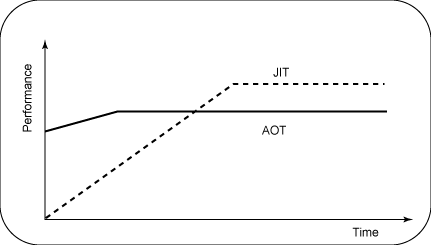
\includegraphics[width=0.7\linewidth]{performanceaotvsjit}
	\caption[Confronto di performance]{Confronto di performance}
	\label{fig:performanceaotvsjit}
\end{figure}

Inizialmente JIT è molto peggiore, perché tutti i metodi sono interpretati. Man mano che vengono compilati però le prestazioni migliorano fino a superare AOT e a raggiungere un picco. AOT, d'altra parte, ha un inizio migliore e si stabilizza più velocemente, ma ad un livello più basso. Nessuna tecnica è adatta per tutti gli scenari: l'una è più forte dove l'altra è più debole. Per le applicazioni real-time, dove l'importante è il determinismo e la prevedibilità, AOT è molto più adatto perché presenta meno variabilità nelle prestazioni.